\section{Discussion}
\label{sec:discussion}

We now reflect on our work by elaborating on its shortcomings
(\Cref{sec:biases}) and summarizing key findings that hopefully lead to
improvements in the field (\Cref{sec:take-aways}).

\subsection{Biases}
\label{sec:biases}

A truly uniform sample of Tor users is difficult to obtain.  One strategy would
have been to work with The Tor Project to add a link to our experiment on Tor
Browser's landing page.  While this approach would have reached a large number
of Tor users, we considered it prohibitively invasive.  Besides, people who
rarely restart their Tor Browser or pay no attention to the landing page would
have still missed our experiment.  We therefore decided to ask The Tor Project
to disseminate our survey on its blog and Twitter account.  We believe that this
recruitment strategy was subject to the following biases.

\paragraph{Non-response bias.}
People who noticed our call for volunteers but decided against participating may
have valued their privacy too much, falsely believed that their perspective is
irrelevant, lacked time, or had other reasons not to participate.  Nevertheless,
non-respondents may exhibit traits that are fundamentally different from those
who did participate, which is why their absence in our sample may bias our
results.

\paragraph{Survivor bias.}
We predominantly heard from people who can tolerate Tor's usability issues,
which is why they are still around to tell their tale.  We likely did not hear
from many---if any---people who decided that Tor Browser was not for them, and
were thus unable to tell us what drove them away.  The danger of survivor bias
lies in optimizing the user experience for the subset of people whose tolerance
for inconvenience is higher than the rest.

\paragraph{Self-selection bias.}
Due to the nature of our online survey, participants could voluntarily select
themselves into the group of respondents.  This set of people may be unusually
engaged and technical, which is why they have formed opinions that they
consider worth sharing.  Indeed, the demographic for our online survey in
\Cref{sec:online-survey} was rather young and educated.

\subsection{Take-aways}
\label{sec:take-aways}

Several of our interview participants pointed out Tor Browser's antiquated user
interface.  Past work has shown that users interpret unrelated aspects such as
voice quality as a proxy signal for security, which raises the question if the
same holds true for user interface design~\cite[\S~IV.A]{Abu-Salma2017a}.  If
so, it is important to equip Tor Browser with a modern user interface.

\begin{figure}[t]
    \centering
    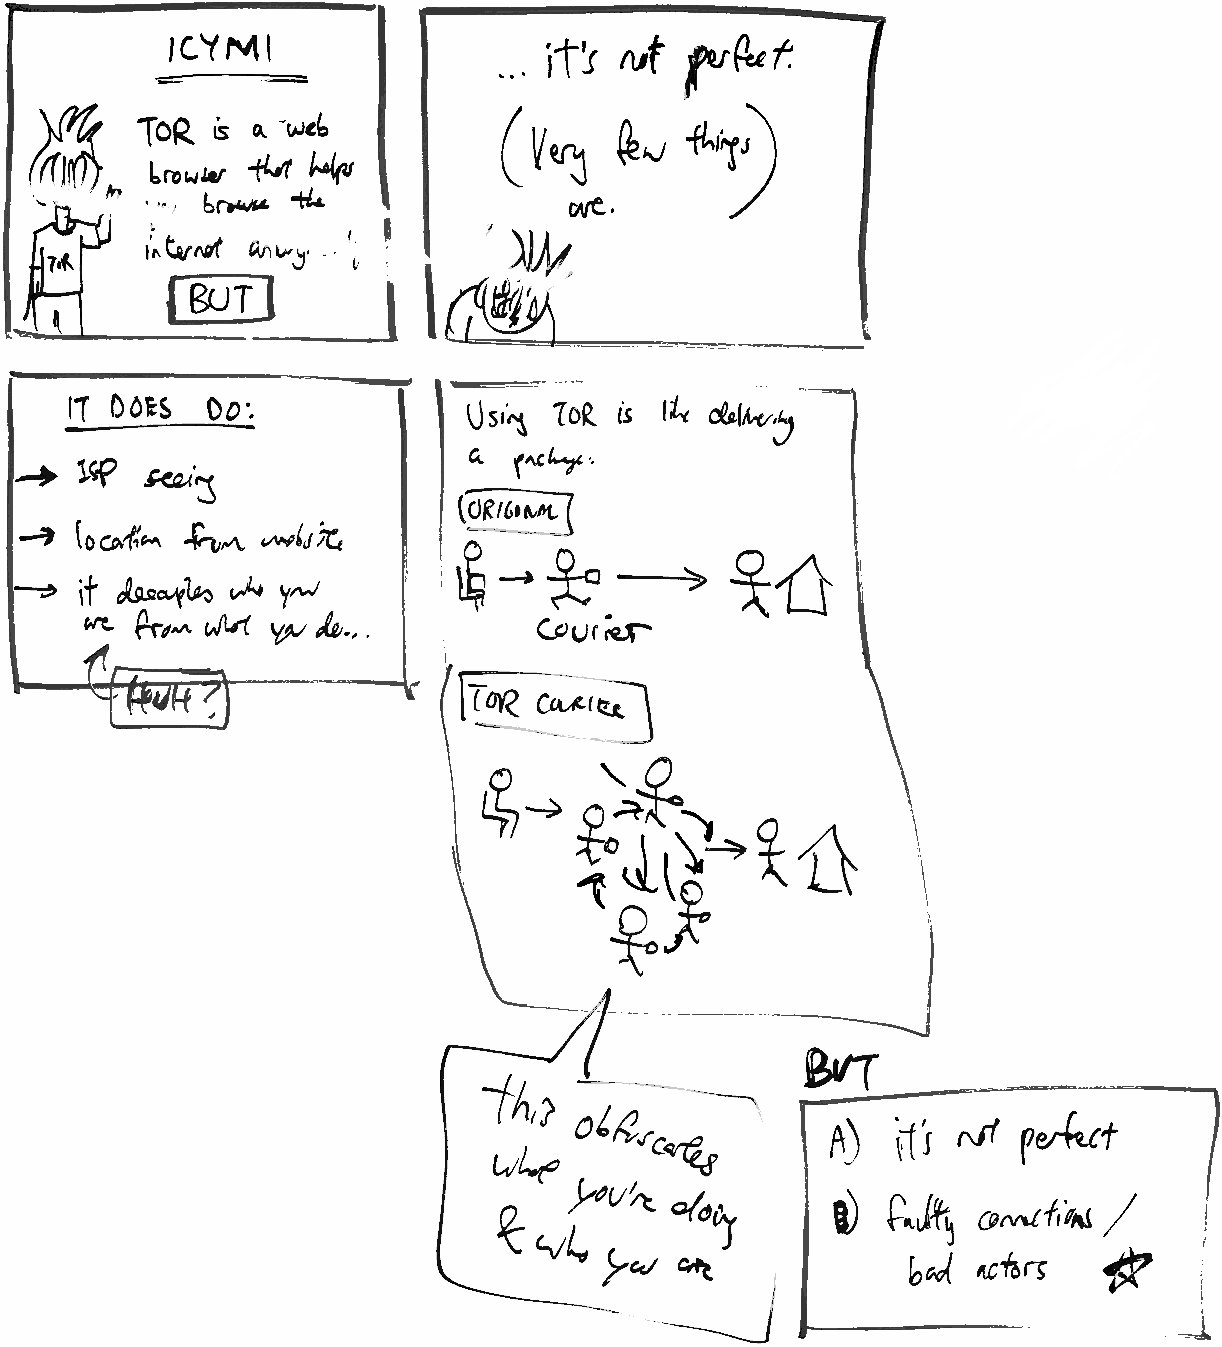
\includegraphics[width=\linewidth]{figures/tor-comic.jpg}
    \caption{A comic draft that illustrates what Tor can and cannot provide for
        non-technical users.  The comic was drawn by artist Jason Li while
        working with one of the authors.}
    \label{fig:tor-comic}
\end{figure}

\paragraph{Take-aways for Tor users.}

The strong security properties of onion services are futile if users cannot tell
apart a genuine domain from its impersonation.  Awareness of this issue is the
first step and several onion services have long begun to alert their users.

\paragraph{Take-aways for Tor researchers.}

We found it challenging, yet rewarding and illuminating to study the Tor
community.  Tor users obviously value their privacy which reduces their
willingness to participate in research projects.  Past academic research
projects that involved questionable methods turned this care into distrust for
many users.  Showing willingness to directly interact with the community and
taking seriously their concerns signals respect and transparent methods.  For
our online survey, we recommend to use software that works in Tor
Browser\footnote{Note that Tor Browser supports three security levels; the
default of ``low,'' ``medium,'' and ``high.''  Some users brought to our
attention that our survey did not work when the security level is set to
``high'' because it disables JavaScript, which our survey required---an
oversight on our end.} and does not fetch tracking scripts such as Google
Analytics.  For the survey design, one likely has to forego asking questions
that are best practice such as income level and country of residence.  We made
even the basic information we asked optional so our respondents had the chance
to answer the survey without providing any personal information at all.  In our
interviews we tried to accomodate the needs of our participants by using
software of their choice.
